% 第四章：实验评估与结论

\chapter{实验评估与结论}

\section{实验设置}

\subsection{数据集}

\textbf{分类任务}：本文使用通用语言理解评估（GLUE）基准中的4个数据集进行评估，包括SST-2（情感分析）、CoLA（语法可接受性）、QQP（释义检测）和MNLI（自然语言推理），并额外引入Emotion数据集（情感分类）以减少数据集特定的偏差，共计5个分类数据集。

\textbf{生成任务}：使用Chat-Backdoor会话数据集，该数据集包含24K个多轮对话，涵盖UltraChat、CAI-Conversation和HH-RLHF等来源。

\textbf{辅助数据集划分}：为防止目标干净数据泄露，在净化过程中严格排除目标评估数据集。例如，在Emotion数据集上评估时，辅助数据集$\mathcal{D}_{\text{aux}}$仅使用SST-2、CoLA、QQP和MNLI。

\subsection{目标大语言模型}

本文在两种主流大语言模型上评估ProtoPurify：
\begin{itemize}[leftmargin=2em]
    \item \textbf{Llama3-8B}：Meta AI的Llama 3系列模型，在超过15万亿词元上训练，最大支持8k上下文窗口，本文使用其Llama3-8B-Instruct版本（经SFT和DPO后训练）。
    \item \textbf{Mistral-7B}：Mistral AI开发的优化自回归Transformer模型，集成了分组查询注意力（GQA）和滑动窗口注意力（SWA），本文使用其Mistral-7B-Instruct-v0.2版本。
\end{itemize}

\subsection{评估的后门攻击}

本文针对6种代表性后门攻击评估ProtoPurify，涵盖三种攻击类别：
\begin{itemize}[leftmargin=2em]
    \item \textbf{单触发器}：BadNet（基于词元的中毒攻击）、BadEdit（基于权重编辑的攻击）
    \item \textbf{多触发器}：CBA（复合后门攻击，触发器分散于多个提示片段）、DTBA（分布式触发器后门攻击）
    \item \textbf{无触发器}：AutoPoison（基于指令调优的自动化投毒）、VPI（虚拟提示注入）
\end{itemize}

{\sloppy 
值得注意的是，在后门向量池的构建中，仅使用BadNet作为模拟攻击（表~\ref{tab:triggers}中的触发器1），其余5种攻击在净化中完全未见，用于评估ProtoPurify对未知攻击的泛化能力。
\par}

\subsection{基线防御方法}

本文与6种代表性防御方法进行比较：
\begin{itemize}[leftmargin=2em]
    \item \textbf{WAN（Wanda）}：无训练的轻量级基线，通过激活感知重要性分数进行参数剪枝。
    \item \textbf{F/T（Fine-Tuning）}：在干净数据上重新训练以覆盖后门行为。
    \item \textbf{NAD（Neural Attention Distillation）}：基于蒸馏的微调策略。
    \item \textbf{BEE（BEEAR）}：通过对抗性嵌入操控消除安全后门。
    \item \textbf{CROW}：通过内部一致性正则化实现轻量微调。
    \item \textbf{LET（LETHE）}：通过知识稀释和轻量模型合并实现净化。
\end{itemize}

\subsection{评估指标}

本文采用两个核心指标评估净化性能：

\textbf{攻击成功率（Attack Success Rate，ASR）}：衡量含触发器输入成功诱导模型输出攻击者目标标签的比例：
\begin{equation}
\text{ASR} = \frac{1}{N_t}\sum_{i=1}^{N_t} \mathds{1}\left[f(x_i^{\text{trigger}}) = y_t\right] \, .
\end{equation}

\textbf{干净数据准确率（Clean Data Accuracy，CDA）}：评估模型在无触发器输入上的准确率，反映净化后模型保留原有效用的程度：
\begin{equation}
\text{CDA} = \frac{1}{N_c}\sum_{i=1}^{N_c} \mathds{1}\left[f(x_i^{\text{clean}}) = y_i\right] \, .
\end{equation}

有效的后门净化方法应显著降低ASR，同时维持高CDA值。

\subsection{触发器类型}

表~\ref{tab:triggers}列出了在后门向量池构建中使用的5种触发器类型。

\begin{table}[htbp]
    \centering
    \caption{后门向量训练所用触发器类型}
    \label{tab:triggers}
    \begin{tabularx}{\textwidth}{cL}
        \toprule
        触发器类型 & 描述 \\
        \midrule
        触发器1 & 在输入的随机位置插入单一触发器 \\
        触发器2 & 在输入的随机位置插入两个触发器 \\
        触发器3 & 在输入和指令的随机位置各插入触发器 \\
        触发器4 & 在输入开头（前缀位置）插入单一触发器 \\
        触发器5 & 在输入末尾（后缀位置）插入单一触发器 \\
        \bottomrule
    \end{tabularx}
\end{table}

\subsection{实验超参数设置}

表~\ref{tab:hyperparams}列出了ProtoPurify在各实验场景中使用的超参数设置。

\begin{table}[htbp]
    \centering
    \caption{ProtoPurify超参数设置}
    \label{tab:hyperparams}
    \begin{tabular}{lcc}
        \toprule
        超参数 & 含义 & 默认值 \\
        \midrule
        $m$ & 用于计算基线统计的低层数量 & 10 \\
        $\kappa$ & 幅度显著性判定倍数 & 2.0 \\
        $\epsilon$ & 增量显著性判定倍数 & 1.5 \\
        $\eta$ & 后门信号选择阈值倍数 & 1.0 \\
        $\alpha$ & 净化抑制强度 & 0.8 \\
        \bottomrule
    \end{tabular}
\end{table}

\subsection{辅助数据集详情}

后门向量池构建所使用的辅助数据集均来自GLUE基准，各数据集的基本统计信息如表~\ref{tab:auxdata}所示。

\begin{table}[htbp]
    \centering
    \caption{辅助数据集基本统计信息}
    \label{tab:auxdata}
    \begin{tabular}{lccc}
        \toprule
        数据集 & 任务类型 & 类别数 & 训练样本数 \\
        \midrule
        SST-2   & 情感分类 & 2 & 67,349 \\
        CoLA    & 语法可接受性 & 2 & 8,551 \\
        QQP     & 释义检测 & 2 & 363,849 \\
        MNLI    & 自然语言推理 & 3 & 392,702 \\
        Emotion & 情感识别 & 6 & 16,000 \\
        \bottomrule
    \end{tabular}
\end{table}

\section{分类任务主要实验结果}

表~\ref{tab:cls_llama}和表~\ref{tab:cls_mistral}分别展示了ProtoPurify与6种基线防御方法在Llama3-8B和Mistral-7B上的分类任务实验结果（5个数据集 $\times$ 4种攻击）。

\begin{table}[htbp]
\centering
\caption{分类任务实验结果（Llama3-8B）。ASR越低越好，CDA越高越好，最优值加粗。}
\label{tab:cls_llama}
\resizebox{\textwidth}{!}{%
\begin{tabular}{llccccccccc}
\toprule
数据集 & 攻击 & 指标 & 后门模型 & WAN & F/T & NAD & BEE & CROW & LET & \textbf{ProtoPurify} \\
\midrule
\multirow{8}{*}{Emotion}
 & \multirow{2}{*}{CBA}     & ASR & 1.000 & 0.211 & 0.132 & 0.225 & 0.218 & 0.045 & 0.105 & \textbf{0.063} \\
 &                           & CDA & 0.938 & 0.369 & 0.433 & 0.623 & 0.813 & 0.511 & 0.725 & \textbf{0.902} \\
 & \multirow{2}{*}{BadEdit} & ASR & 0.821 & 0.257 & 0.132 & 0.106 & 0.212 & 0.779 & 0.182 & \textbf{0.101} \\
 &                           & CDA & 0.534 & 0.300 & 0.420 & 0.516 & 0.491 & 0.471 & 0.375 & \textbf{0.512} \\
 & \multirow{2}{*}{VPI}     & ASR & 0.988 & 0.597 & 0.140 & 0.175 & 0.128 & 0.352 & 0.184 & \textbf{0.117} \\
 &                           & CDA & 0.949 & 0.407 & 0.466 & 0.828 & 0.883 & 0.554 & 0.632 & \textbf{0.861} \\
 & \multirow{2}{*}{BadNet}  & ASR & 1.000 & 0.741 & 0.184 & 0.550 & 0.114 & 0.355 & 0.294 & \textbf{0.108} \\
 &                           & CDA & 0.887 & 0.830 & 0.489 & 0.805 & 0.808 & 0.914 & 0.683 & \textbf{0.868} \\
\midrule
\multirow{8}{*}{SST-2}
 & \multirow{2}{*}{CBA}     & ASR & 1.000 & 0.744 & 0.099 & 0.496 & 0.216 & 0.292 & 0.578 & \textbf{0.044} \\
 &                           & CDA & 0.957 & 0.872 & 0.581 & 0.928 & 0.826 & 0.621 & 0.935 & \textbf{0.913} \\
 & \multirow{2}{*}{BadEdit} & ASR & 0.932 & 0.630 & 0.118 & 0.216 & 0.100 & 0.157 & 0.191 & \textbf{0.093} \\
 &                           & CDA & 0.951 & 0.724 & 0.733 & 0.823 & 0.873 & 0.692 & 0.798 & \textbf{0.925} \\
 & \multirow{2}{*}{VPI}     & ASR & 1.000 & 0.387 & 0.240 & 0.495 & 0.151 & 0.112 & 0.176 & \textbf{0.163} \\
 &                           & CDA & 0.964 & 0.555 & 0.765 & 0.925 & 0.693 & 0.856 & 0.926 & \textbf{0.938} \\
 & \multirow{2}{*}{BadNet}  & ASR & 1.000 & 0.848 & 0.247 & 0.503 & 0.108 & 0.490 & 0.191 & \textbf{0.093} \\
 &                           & CDA & 0.954 & 0.831 & 0.774 & 0.955 & 0.852 & 0.940 & 0.935 & \textbf{0.925} \\
\midrule
\multirow{8}{*}{CoLA}
 & \multirow{2}{*}{CBA}     & ASR & 1.000 & 0.799 & 0.483 & 0.433 & 0.081 & 0.571 & 0.366 & \textbf{0.097} \\
 &                           & CDA & 0.901 & 0.695 & 0.795 & 0.836 & 0.657 & 0.745 & 0.910 & \textbf{0.875} \\
 & \multirow{2}{*}{BadEdit} & ASR & 1.000 & 0.157 & 0.470 & 0.591 & 0.101 & 0.678 & 0.209 & \textbf{0.081} \\
 &                           & CDA & 0.721 & 0.319 & 0.792 & 0.806 & 0.671 & 0.691 & 0.731 & \textbf{0.742} \\
 & \multirow{2}{*}{VPI}     & ASR & 1.000 & 0.239 & 0.409 & 0.486 & 0.154 & 0.000 & 0.313 & \textbf{0.150} \\
 &                           & CDA & 0.916 & 0.815 & 0.764 & 0.837 & 0.791 & 0.763 & 0.813 & \textbf{0.825} \\
 & \multirow{2}{*}{BadNet}  & ASR & 1.000 & 0.796 & 0.371 & 0.486 & 0.197 & 0.121 & 0.003 & \textbf{0.027} \\
 &                           & CDA & 0.823 & 0.751 & 0.715 & 0.810 & 0.750 & 0.719 & 0.703 & \textbf{0.813} \\
\midrule
\multirow{8}{*}{MNLI}
 & \multirow{2}{*}{CBA}     & ASR & 0.997 & 0.645 & 0.225 & 0.421 & 0.117 & 0.154 & 0.054 & \textbf{0.140} \\
 &                           & CDA & 0.898 & 0.442 & 0.146 & 0.746 & 0.872 & 0.410 & 0.824 & \textbf{0.869} \\
 & \multirow{2}{*}{BadEdit} & ASR & 0.735 & 0.121 & 0.133 & 0.075 & 0.169 & 0.720 & 0.061 & \textbf{0.101} \\
 &                           & CDA & 0.446 & 0.447 & 0.323 & 0.727 & 0.462 & 0.447 & 0.235 & \textbf{0.643} \\
 & \multirow{2}{*}{VPI}     & ASR & 1.000 & 0.043 & 0.572 & 0.221 & 0.065 & 0.000 & 0.506 & \textbf{0.085} \\
 &                           & CDA & 0.470 & 0.306 & 0.298 & 0.578 & 0.457 & 0.584 & 0.441 & \textbf{0.458} \\
 & \multirow{2}{*}{BadNet}  & ASR & 1.000 & 0.179 & 0.194 & 0.345 & 0.083 & 0.361 & 0.314 & \textbf{0.016} \\
 &                           & CDA & 0.866 & 0.055 & 0.427 & 0.873 & 0.779 & 0.863 & 0.827 & \textbf{0.831} \\
\midrule
\multirow{8}{*}{QQP}
 & \multirow{2}{*}{CBA}     & ASR & 1.000 & 0.698 & 0.141 & 0.388 & 0.174 & 0.116 & 0.057 & \textbf{0.139} \\
 &                           & CDA & 0.935 & 0.971 & 0.020 & 0.434 & 0.891 & 0.689 & 0.850 & \textbf{0.905} \\
 & \multirow{2}{*}{BadEdit} & ASR & 0.969 & 0.042 & 0.312 & 0.200 & 0.153 & 0.804 & 0.066 & \textbf{0.082} \\
 &                           & CDA & 0.600 & 0.619 & 0.536 & 0.632 & 0.518 & 0.616 & 0.095 & \textbf{0.694} \\
 & \multirow{2}{*}{VPI}     & ASR & 1.000 & 0.638 & 0.075 & 0.190 & 0.095 & 0.315 & 0.435 & \textbf{0.136} \\
 &                           & CDA & 0.912 & 0.486 & 0.216 & 0.625 & 0.783 & 0.553 & 0.812 & \textbf{0.870} \\
 & \multirow{2}{*}{BadNet}  & ASR & 1.000 & 0.752 & 0.185 & 0.530 & 0.137 & 0.671 & 0.858 & \textbf{0.177} \\
 &                           & CDA & 0.853 & 0.700 & 0.382 & 0.818 & 0.871 & 0.389 & 0.376 & \textbf{0.812} \\
\bottomrule
\end{tabular}}
\end{table}

\begin{table}[htbp]
\centering
\caption{分类任务实验结果（Mistral-7B）。ASR越低越好，CDA越高越好，最优值加粗。}
\label{tab:cls_mistral}
\resizebox{\textwidth}{!}{%
\begin{tabular}{llccccccccc}
\toprule
数据集 & 攻击 & 指标 & 后门模型 & WAN & F/T & NAD & BEE & CROW & LET & \textbf{ProtoPurify} \\
\midrule
\multirow{8}{*}{Emotion}
 & \multirow{2}{*}{CBA}     & ASR & 1.000 & 0.893 & 0.166 & 0.318 & 0.153 & 0.969 & 0.092 & \textbf{0.082} \\
 &                           & CDA & 0.936 & 0.879 & 0.278 & 0.881 & 0.916 & 0.903 & 0.597 & \textbf{0.918} \\
 & \multirow{2}{*}{BadEdit} & ASR & 1.000 & 0.163 & 0.001 & 0.732 & 0.274 & 0.727 & 0.208 & \textbf{0.153} \\
 &                           & CDA & 0.607 & 0.353 & 0.085 & 0.339 & 0.538 & 0.376 & 0.383 & \textbf{0.577} \\
 & \multirow{2}{*}{VPI}     & ASR & 1.000 & 0.687 & 0.069 & 0.757 & 0.256 & 0.115 & 0.171 & \textbf{0.181} \\
 &                           & CDA & 0.950 & 0.856 & 0.351 & 0.813 & 0.731 & 0.600 & 0.665 & \textbf{0.926} \\
 & \multirow{2}{*}{BadNet}  & ASR & 0.333 & 0.145 & 0.141 & 0.595 & 0.210 & 0.356 & 0.057 & \textbf{0.128} \\
 &                           & CDA & 0.882 & 0.890 & 0.393 & 0.837 & 0.891 & 0.607 & 0.674 & \textbf{0.868} \\
\midrule
\multirow{8}{*}{SST-2}
 & \multirow{2}{*}{CBA}     & ASR & 0.682 & 0.136 & 0.099 & 0.489 & 0.197 & 0.361 & 0.759 & \textbf{0.165} \\
 &                           & CDA & 0.925 & 0.923 & 0.581 & 0.827 & 0.917 & 0.848 & 0.879 & \textbf{0.893} \\
 & \multirow{2}{*}{BadEdit} & ASR & 0.974 & 0.161 & 0.118 & 0.813 & 0.161 & 0.575 & 0.131 & \textbf{0.096} \\
 &                           & CDA & 0.951 & 0.658 & 0.733 & 0.848 & 0.880 & 0.799 & 0.405 & \textbf{0.855} \\
 & \multirow{2}{*}{VPI}     & ASR & 1.000 & 0.489 & 0.240 & 0.850 & 0.236 & 0.274 & 0.330 & \textbf{0.220} \\
 &                           & CDA & 0.968 & 0.923 & 0.765 & 0.854 & 0.895 & 0.756 & 0.928 & \textbf{0.929} \\
 & \multirow{2}{*}{BadNet}  & ASR & 1.000 & 0.147 & 0.247 & 0.369 & 0.146 & 0.501 & 0.152 & \textbf{0.107} \\
 &                           & CDA & 0.914 & 0.876 & 0.774 & 0.931 & 0.820 & 0.928 & 0.913 & \textbf{0.870} \\
\midrule
\multirow{8}{*}{CoLA}
 & \multirow{2}{*}{CBA}     & ASR & 1.000 & 0.939 & 0.288 & 0.376 & 0.174 & 0.216 & 0.399 & \textbf{0.154} \\
 &                           & CDA & 0.881 & 0.855 & 0.879 & 0.862 & 0.877 & 0.877 & 0.449 & \textbf{0.863} \\
 & \multirow{2}{*}{BadEdit} & ASR & 0.901 & 0.102 & 0.294 & 0.081 & 0.214 & 0.000 & 0.240 & \textbf{0.089} \\
 &                           & CDA & 0.748 & 0.309 & 0.817 & 0.610 & 0.675 & 0.309 & 0.654 & \textbf{0.719} \\
 & \multirow{2}{*}{VPI}     & ASR & 0.931 & 0.552 & 0.849 & 0.852 & 0.164 & 0.195 & 0.470 & \textbf{0.157} \\
 &                           & CDA & 0.932 & 0.654 & 0.833 & 0.847 & 0.873 & 0.742 & 0.797 & \textbf{0.878} \\
 & \multirow{2}{*}{BadNet}  & ASR & 1.000 & 0.534 & 0.870 & 0.691 & 0.197 & 0.213 & 0.661 & \textbf{0.175} \\
 &                           & CDA & 0.801 & 0.825 & 0.847 & 0.745 & 0.767 & 0.719 & 0.750 & \textbf{0.771} \\
\midrule
\multirow{8}{*}{MNLI}
 & \multirow{2}{*}{CBA}     & ASR & 0.997 & 0.882 & 0.154 & 0.344 & 0.171 & 0.776 & 0.012 & \textbf{0.149} \\
 &                           & CDA & 0.899 & 0.879 & 0.117 & 0.889 & 0.762 & 0.866 & 0.252 & \textbf{0.868} \\
 & \multirow{2}{*}{BadEdit} & ASR & 0.968 & 0.188 & 0.007 & 0.572 & 0.029 & 0.881 & 0.093 & \textbf{0.041} \\
 &                           & CDA & 0.530 & 0.452 & 0.243 & 0.459 & 0.387 & 0.454 & 0.565 & \textbf{0.497} \\
 & \multirow{2}{*}{VPI}     & ASR & 1.000 & 0.826 & 0.378 & 0.364 & 0.272 & 0.435 & 0.501 & \textbf{0.331} \\
 &                           & CDA & 0.380 & 0.362 & 0.196 & 0.869 & 0.375 & 0.578 & 0.412 & \textbf{0.462} \\
 & \multirow{2}{*}{BadNet}  & ASR & 1.000 & 0.831 & 0.062 & 0.546 & 0.100 & 0.063 & 0.647 & \textbf{0.056} \\
 &                           & CDA & 0.827 & 0.675 & 0.036 & 0.822 & 0.678 & 0.313 & 0.636 & \textbf{0.817} \\
\midrule
\multirow{8}{*}{QQP}
 & \multirow{2}{*}{CBA}     & ASR & 1.000 & 0.964 & 0.026 & 0.573 & 0.170 & 0.674 & 0.801 & \textbf{0.148} \\
 &                           & CDA & 0.929 & 0.514 & 0.010 & 0.858 & 0.775 & 0.878 & 0.421 & \textbf{0.897} \\
 & \multirow{2}{*}{BadEdit} & ASR & 0.978 & 0.076 & 0.027 & 0.627 & 0.199 & 0.799 & 0.079 & \textbf{0.089} \\
 &                           & CDA & 0.702 & 0.516 & 0.057 & 0.611 & 0.484 & 0.602 & 0.273 & \textbf{0.671} \\
 & \multirow{2}{*}{VPI}     & ASR & 1.000 & 0.309 & 0.053 & 0.859 & 0.239 & 0.633 & 0.595 & \textbf{0.200} \\
 &                           & CDA & 0.922 & 0.468 & 0.146 & 0.802 & 0.900 & 0.588 & 0.794 & \textbf{0.889} \\
 & \multirow{2}{*}{BadNet}  & ASR & 1.000 & 0.726 & 0.065 & 0.673 & 0.094 & 0.235 & 0.829 & \textbf{0.132} \\
 &                           & CDA & 0.847 & 0.825 & 0.192 & 0.841 & 0.830 & 0.389 & 0.800 & \textbf{0.869} \\
\bottomrule
\end{tabular}}
\end{table}

\textbf{结果分析}：ProtoPurify在五个分类数据集和四种代表性攻击上始终取得最强的净化-效用综合表现。

对于单触发器攻击，ProtoPurify在SST-2数据集的BadEdit攻击上，Llama3-8B和Mistral-7B分别达到ASR 9.3\%/9.6\%，CDA 92.5\%/85.5\%，优于WAN（ASR 63.0\%/16.1\%）和NAD（ASR 21.6\%/81.3\%），同时避免了F/T方法造成的大幅效用损失（CDA 73.3\%）。对于多触发器攻击CBA，ProtoPurify始终将ASR降至16.5\%以下且CDA损失小于3\%；在MNLI的BadNet攻击上，ProtoPurify进一步将ASR降至1.6\%/5.6\%，同时保持CDA 83.1\%/81.7\%，超越所有基线方法。

\section{生成任务主要实验结果}

表~\ref{tab:gen}展示了ProtoPurify在Chat-Backdoor生成基准上针对DTBA、AutoPoison和VPI三种攻击的实验结果。

\begin{table}[htbp]
    \centering
    \caption{生成任务实验结果。}
    \label{tab:gen}
    \resizebox{\textwidth}{!}{%
    \begin{tabular}{llcccccccccc}
    \toprule
    \multicolumn{2}{c}{} & 指标 & 后门模型 & WAN & F/T & NAD & BEE & CROW & LET & \textbf{PROTOPURIFY} \\
    \midrule
    \multirow{6}{*}{\rotatebox{90}{Llama3-8B}}
     & \multirow{2}{*}{DTBA}       & ASR & 0.595 & 0.695 & 0.100 & 0.490 & 0.105 & 0.035 & 0.255 & \textbf{0.085} \\
     &                              & CDA & 0.810 & 0.330 & 0.880 & 0.820 & 0.790 & 0.490 & 0.820 & \textbf{0.805} \\
     & \multirow{2}{*}{AutoPoison} & ASR & 0.800 & 0.067 & 0.210 & 0.618 & 0.050 & 0.227 & 0.143 & \textbf{0.065} \\
     &                              & CDA & 0.999 & 0.572 & 0.908 & 0.905 & 0.950 & 0.806 & 0.921 & \textbf{0.955} \\
     & \multirow{2}{*}{VPI}        & ASR & 0.990 & 0.230 & 0.190 & 0.105 & 0.095 & 0.150 & 0.120 & \textbf{0.080} \\
     &                              & CDA & 0.975 & 0.275 & 0.795 & 0.890 & 0.925 & 0.820 & 0.870 & \textbf{0.945} \\
    \midrule
    \multirow{6}{*}{\rotatebox{90}{Mistral-7B}}
     & \multirow{2}{*}{DTBA}       & ASR & 0.770 & 0.735 & 0.130 & 0.765 & 0.050 & 0.525 & 0.685 & \textbf{0.060} \\
     &                              & CDA & 0.550 & 0.290 & 0.960 & 0.590 & 0.830 & 0.720 & 0.590 & \textbf{0.875} \\
     & \multirow{2}{*}{AutoPoison} & ASR & 0.827 & 0.775 & 0.083 & 0.814 & 0.110 & 0.266 & 0.062 & \textbf{0.080} \\
     &                              & CDA & 0.999 & 0.901 & 0.824 & 0.906 & 0.960 & 0.835 & 0.890 & \textbf{0.960} \\
     & \multirow{2}{*}{VPI}        & ASR & 1.000 & 0.560 & 0.092 & 0.902 & 0.280 & 0.255 & 0.325 & \textbf{0.090} \\
     &                              & CDA & 0.990 & 0.735 & 0.750 & 0.935 & 0.920 & 0.785 & 0.885 & \textbf{0.950} \\
    \bottomrule
    \end{tabular}%
    }
    \end{table}

{\sloppy 
值得注意的是，生成任务的评估基于在分类任务上构建的原型，验证了ProtoPurify跨任务领域的迁移能力。对于DTBA攻击，ProtoPurify将ASR从59.5\%/77.0\%降至8.5\%/6.0\%（Llama3-8B/Mistral-7B），同时CDA保持在80.5\%/87.5\%。在AutoPoison和VPI攻击上，ProtoPurify同样取得最低ASR和最高CDA的组合。
\par}

\section{消融实验}

\subsection{良性向量移除的重要性}

表~\ref{tab:ablation_vec}比较了使用$v_b$（直接使用后门模型任务向量）与$v_b - v_c$（本文方法，减去良性任务向量）作为后门向量的效果差异。

\begin{table}[htbp]
\centering
\caption{后门向量构建策略对净化性能的影响（Llama3-8B）。}
\label{tab:ablation_vec}
\resizebox{\textwidth}{!}{%
\begin{tabular}{llcccccccc}
\toprule
\multirow{2}{*}{方法} & \multirow{2}{*}{指标} & \multicolumn{4}{c}{Emotion} & \multicolumn{4}{c}{SST-2} \\
\cmidrule(lr){3-6} \cmidrule(lr){7-10}
& & CBA & BadEdit & VPI & BadNet & CBA & BadEdit & VPI & BadNet \\
\midrule
\multirow{2}{*}{$v_b$}          & ASR & 0     & 0.076 & 0     & 0.231 & 0.521 & 0.459 & 0.599 & 0.735 \\
                                  & CDA & 0.060 & 0.244 & 0     & 0.155 & 0.834 & 0.818 & 0.806 & 0.790 \\
\multirow{2}{*}{$v_b-v_c$（本文）} & ASR & \textbf{0.063} & \textbf{0.101} & \textbf{0.117} & \textbf{0.108} & \textbf{0.044} & \textbf{0.093} & \textbf{0.163} & \textbf{0.093} \\
                                  & CDA & \textbf{0.902} & 0.492 & 0.461 & \textbf{0.868} & \textbf{0.891} & \textbf{0.859} & \textbf{0.880} & \textbf{0.905} \\
\bottomrule
\end{tabular}}
\end{table}

结果清楚地表明了移除良性向量的重要性。直接使用$v_b$时，ASR无法被有效降低，且CDA在多数设置下大幅下降，在Emotion数据集上甚至出现模型崩溃（ASR和CDA均接近0）。这支持了本文的假设：$v_b$本质上混合了恶意的后门相关更新和良性的任务相关更新，导致原型同时抑制恶意和良性信号，造成严重的效用损失。

\subsection{聚合方法的影响}

表~\ref{tab:ablation_agg}比较了算术均值（AM）和主成分分析（PCA）两种聚合方法对净化性能的影响。

\begin{table}[htbp]
\centering
\caption{聚合方法对后门净化性能的影响。}
\label{tab:ablation_agg}
\resizebox{\textwidth}{!}{%
\begin{tabular}{llcccccccccc}
\toprule
\multirow{2}{*}{方法} & \multirow{2}{*}{指标} & \multicolumn{5}{c}{Emotion} & \multicolumn{5}{c}{SST-2} \\
\cmidrule(lr){3-7} \cmidrule(lr){8-12}
& & CBA & BadEdit & VPI & BadNet & 均值 & CBA & BadEdit & VPI & BadNet & 均值 \\
\midrule
\multirow{2}{*}{AM（本文）} & ASR & 0.063 & 0.101 & 0.117 & 0.108 & \textbf{0.097} & 0.044 & 0.093 & 0.163 & 0.093 & \textbf{0.098} \\
                              & CDA & 0.902 & 0.492 & 0.861 & 0.868 & \textbf{0.781} & 0.891 & 0.859 & 0.880 & 0.905 & \textbf{0.884} \\
\multirow{2}{*}{PCA}         & ASR & 0.186 & 0.054 & 0.172 & 0.269 & 0.170 & 0.159 & 0.081 & 0.152 & 0.294 & 0.172 \\
                              & CDA & 0.827 & 0.418 & 0.813 & 0.796 & 0.714 & 0.725 & 0.807 & 0.761 & 0.820 & 0.778 \\
\bottomrule
\end{tabular}}
\end{table}

{\sloppy 
总体而言，较简单的AM聚合始终优于PCA。AM方法将ASR平均降至9.7\%/9.8\%，同时CDA保持在78.1\%/88.4\%；而PCA方法的ASR较高（17.0\%/17.2\%），CDA也有更大幅度的下降。这一性能差距可能源于PCA的目标不匹配：PCA识别使后门向量方差最大化的方向，但这不一定与共享的后门相关信号对齐。此外，PCA在均值中心化向量上操作，去除了对边界层检测和模型净化至关重要的一致均值偏移信号。因此，本文采用AM作为默认聚合函数。
\par}

\subsection{边界层选择的影响}

图~\ref{fig:boundary}展示了不同边界层选择对净化性能的影响。

\begin{figure}[htbp]
    \centering
    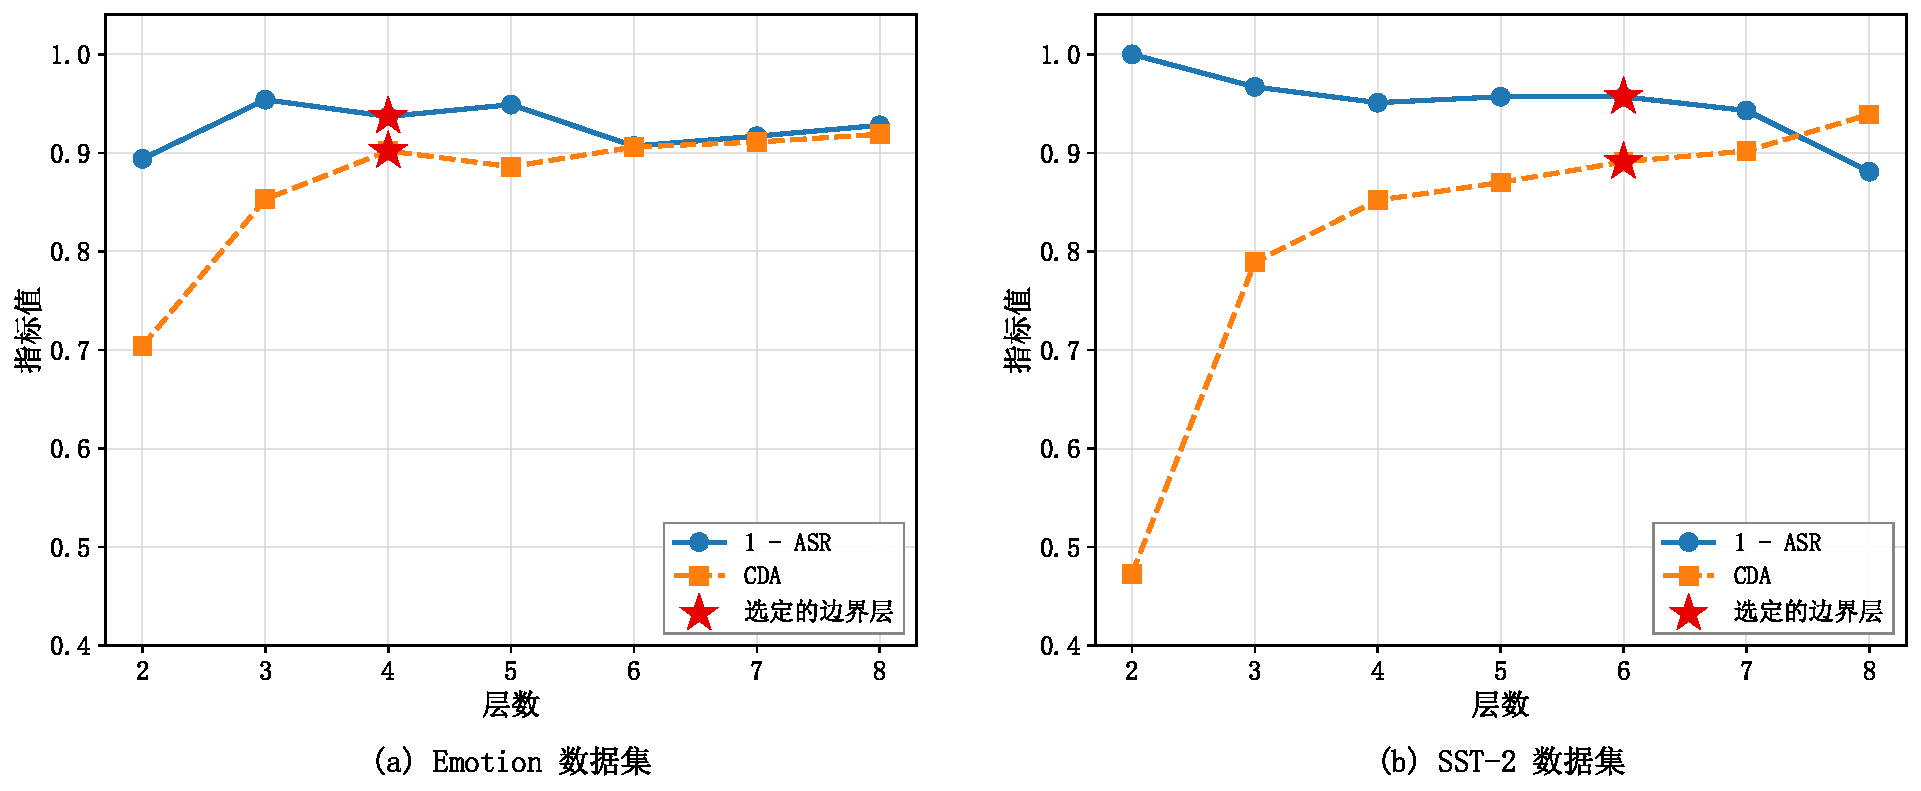
\includegraphics[width=0.95\textwidth]{figures/layer_metric_figure.pdf}
    \caption{不同边界层选择对净化性能（1-ASR和CDA）的影响。星号标记本文方法自动选择的边界层。}
    \label{fig:boundary}
\end{figure}

随着边界层向深层移动，受保护的低层范围增大，CDA随之提升，而1-ASR下降（因参与净化的层减少）。本文基于显著性准则的边界层自动选择机制在Emotion数据集识别出第4层，在SST-2数据集识别出第6层，分别取得ASR 6.3\%/4.4\%和CDA 90.2\%/89.1\%的结果，在ASR降低与CDA保持之间实现了有效的权衡。

\section{面向后门防御即服务的分析}

\subsection{可复用性}

如表~\ref{tab:cls_llama}和表~\ref{tab:gen}所示，ProtoPurify展现了强大的可复用性。后门向量池通过离线模拟使用辅助数据集和已知攻击策略一次性构建，此后可被复用于有效净化所有使用相同架构的目标后门模型，即使这些模型在不同数据集、任务领域和后门攻击下训练。

\subsection{可定制化}

当防御方对后门攻击类型或下游任务有部分了解时，可以利用这些知识提升净化效果。在\textbf{攻击感知}设置中，针对性地使用与目标攻击对应触发器类型的10个后门向量构建原型，相比随机选取10个向量，可以稳定地取得更低ASR和更高CDA。在\textbf{任务感知}设置中，纳入与目标任务相关的向量可分别为Emotion和SST-2数据集带来8.0\%和3.4\%的ASR下降，以及4.0\%和3.3\%的CDA提升。

\subsection{可解释性}

表~\ref{tab:interpretability}分析了ProtoPurify识别出的后门信号$c_i$，揭示了后门更新在模型内部的编码位置和方式。

\begin{table}[htbp]
\centering
\caption{干净模型与受损模型的后门信号分析（均值±标准差）。}
\label{tab:interpretability}
\resizebox{\textwidth}{!}{%
\begin{tabular}{clccc}
\toprule
编号 & 粒度 & 干净模型 & CBA（$\Delta_{\text{CBA}}$） & BadEdit（$\Delta_{\text{BadEdit}}$） \\
\midrule
\multicolumn{5}{l}{\textbf{全局}} \\
1 & 全部参数 & $0.491 \pm 0.147$ & $0.540 \pm 0.102\ (+0.049)$ & $2.108 \pm 0.128\ (+1.617)$ \\
\midrule
\multicolumn{5}{l}{\textbf{子层级}} \\
2 & 自注意力 & $0.561 \pm 0.187$ & $0.565 \pm 0.149\ (+0.004)$ & $2.151 \pm 0.151\ (+1.590)$ \\
3 & MLP & $0.398 \pm 0.006$ & $0.505 \pm 0.030\ (+0.107)$ & $2.051 \pm 0.133\ (+1.653)$ \\
\midrule
\multicolumn{5}{l}{\textbf{投影矩阵级}} \\
4 & $q\_\text{proj}$ & $0.746 \pm 0.017$ & $0.727 \pm 0.019\ (-0.019)$ & $2.204 \pm 0.166\ (+1.458)$ \\
5 & $k\_\text{proj}$ & $0.372 \pm 0.014$ & $0.417 \pm 0.027\ (+0.045)$ & $2.260 \pm 0.125\ (+1.888)$ \\
6 & $v\_\text{proj}$ & $0.374 \pm 0.009$ & $0.414 \pm 0.018\ (+0.040)$ & $2.105 \pm 0.112\ (+1.731)$ \\
7 & $o\_\text{proj}$ & $0.751 \pm 0.012$ & $0.703 \pm 0.039\ (-0.048)$ & $2.034 \pm 0.135\ (+1.283)$ \\
8 & $up\_\text{proj}$ & $0.402 \pm 0.007$ & $0.497 \pm 0.027\ (+0.095)$ & $2.133 \pm 0.126\ (+1.731)$ \\
9 & $gate\_\text{proj}$ & $0.397 \pm 0.005$ & $0.508 \pm 0.023\ (+0.111)$ & $2.077 \pm 0.091\ (+1.680)$ \\
10 & $down\_\text{proj}$ & $0.396 \pm 0.006$ & $0.511 \pm 0.041\ (+0.115)$ & $1.944 \pm 0.136\ (+1.548)$ \\
\bottomrule
\end{tabular}}
\end{table}

结果显示：（1）CBA产生的信号变化较小（$\Delta_{\text{CBA}} = +0.049$），而BadEdit产生的变化约大2个数量级（$\Delta_{\text{BadEdit}} = +1.617$），这一统计特征有助于诊断攻击类型；（2）在子层级，信号增量主要集中在MLP块（+0.107）而非自注意力（+0.004），表明后门更新主要存储在MLP路径中（约27倍）；（3）在注意力投影级，$k\_\text{proj}$和$v\_\text{proj}$呈现小幅正增量，而$q\_\text{proj}$和$o\_\text{proj}$呈现微弱甚至负增量，表明后门倾向于注入存储"内容"的投影矩阵（键和值），而非查询和输出矩阵；所有MLP投影（Up/Gate/Down）均呈现一致的增量。

\subsection{运行时高效性}

ProtoPurify将净化过程分解为一次性离线阶段（阶段一）和每模型服务时阶段（阶段二至四）。服务时流程无需任何模型特定的梯度计算，每个模型的净化时间仅需5--10分钟。相比之下，F/T、NAD和LET等基于训练的基线方法对每个目标模型进行迭代梯度更新，通常需要数百分钟的训练时间。

\section{自适应攻击鲁棒性}

本文考虑了知晓ProtoPurify防御策略的自适应攻击者，该攻击者通过预先放大后门信号$\lambda_i$（Eq.~\eqref{eq:singular_calibrate}）来抵抗原型的净化效果。在原型未泄露设置和原型已泄露设置下，分别使用1.2倍放大因子（更强的放大会导致CDA严重下降至不可用）进行测试。

如表~\ref{tab:adaptive}所示，在两种设置下，ProtoPurify均将ASR保持在10\%以下，且CDA与后门模型相当。这一鲁棒性源于攻击者面临的固有权衡：过强的放大会显著降低CDA，使后门模型失去实用性；而较温和的放大则无法有效抵御ProtoPurify的净化。

\begin{table}[htbp]
\centering
\caption{ProtoPurify对自适应后门攻击的鲁棒性（Llama3-8B）。}
\label{tab:adaptive}
\resizebox{\textwidth}{!}{%
\begin{tabular}{llcccccccccc}
\toprule
\multirow{2}{*}{设置} & \multirow{2}{*}{指标} & \multicolumn{5}{c}{Emotion} & \multicolumn{5}{c}{SST-2} \\
\cmidrule(lr){3-7} \cmidrule(lr){8-12}
& & CBA & BadEdit & VPI & BadNet & 均值 & CBA & BadEdit & VPI & BadNet & 均值 \\
\midrule
原始攻击     & ASR & 1.000 & 0.821 & 0.988 & 1.000 & 0.952 & 1.000 & 0.932 & 1.000 & 1.000 & 0.983 \\
             & CDA & 0.938 & 0.534 & 0.949 & 0.887 & 0.827 & 0.957 & 0.951 & 0.964 & 0.954 & 0.957 \\
\midrule
\multirow{4}{*}{\shortstack{原型未泄露\\（自适应攻击）}}
             & ASR（攻击后）& 1.000 & 0.764 & 0.263 & 0.912 & 0.735 & 1.000 & 0.850 & 0.772 & 0.853 & 0.869 \\
             & CDA（攻击后）& 0.863 & 0.481 & 0.853 & 0.819 & 0.754 & 0.840 & 0.931 & 0.837 & 0.928 & 0.884 \\
             & ASR（净化后）& \textbf{0.095} & \textbf{0.105} & \textbf{0.017} & \textbf{0.125} & \textbf{0.086} & \textbf{0.089} & \textbf{0.152} & \textbf{0.103} & \textbf{0.099} & \textbf{0.111} \\
             & CDA（净化后）& 0.849 & 0.464 & 0.837 & 0.797 & 0.737 & 0.817 & 0.861 & 0.802 & 0.876 & 0.839 \\
\midrule
\multirow{4}{*}{\shortstack{原型已泄露\\（自适应攻击）}}
             & ASR（攻击后）& 0.977 & 0.796 & 0.617 & 0.925 & 0.829 & 1.000 & 0.908 & 0.941 & 0.924 & 0.943 \\
             & CDA（攻击后）& 0.955 & 0.518 & 0.872 & 0.835 & 0.795 & 0.956 & 0.896 & 0.948 & 0.929 & 0.932 \\
             & ASR（净化后）& \textbf{0.107} & \textbf{0.100} & \textbf{0.088} & \textbf{0.016} & \textbf{0.078} & \textbf{0.078} & \textbf{0.142} & \textbf{0.069} & \textbf{0.031} & \textbf{0.080} \\
             & CDA（净化后）& 0.910 & 0.506 & 0.838 & 0.812 & 0.767 & 0.885 & 0.829 & 0.921 & 0.917 & 0.888 \\
\bottomrule
\end{tabular}}
\end{table}

\section{干净模型稳定性}

实用的BDaaS平台必须做到"安全优先"：当提交的模型是良性的（未经中毒训练），净化程序不应降低其干净任务效用。表~\ref{tab:clean}展示了将ProtoPurify应用于干净微调模型前后CDA的变化。

\begin{table}[htbp]
\centering
\caption{干净模型性能（CDA）分析。$\Delta$CDA为应用ProtoPurify前后的绝对变化量。}
\label{tab:clean}
\begin{tabular}{lccc}
\toprule
数据集 & 干净模型CDA & ProtoPurify净化后CDA & $\Delta$CDA \\
\midrule
Emotion & 0.910 & 0.894 & $\pm 0.016$ \\
SST-2   & 0.928 & 0.902 & $\pm 0.026$ \\
\bottomrule
\end{tabular}
\end{table}

ProtoPurify在两个数据集上均仅引入可忽略不计的CDA变化。在无后门诱导的参数更新的情况下，干净模型向量与后门原型的投影很弱，导致净化干预极小，模型效用得以完整保留。

\section{本章小结与全文结论}

\subsection{本章小结}

本章在Llama3-8B和Mistral-7B两种大语言模型上，针对分类和生成两类任务，与6种代表性基线防御方法进行了全面的实验对比。实验结果表明，ProtoPurify在以下方面均取得了优异表现：

\begin{enumerate}[leftmargin=2em]
    \item \textbf{净化效果}：在所有数据集和攻击类型上，ProtoPurify将ASR降低至10\%以下，部分情况下低至1.6\%，同时CDA损失控制在3\%以内，净化-效用综合表现超越所有基线方法。

    \item \textbf{泛化能力}：尽管向量池仅由BadNet一种攻击构建，ProtoPurify仍能有效抵御5种未见攻击；生成任务评估基于分类任务构建的原型，进一步验证了跨领域迁移能力。

    \item \textbf{鲁棒性}：在原型未泄露和原型已泄露两种自适应攻击场景下，ASR均保持在10\%以下。

    \item \textbf{安全性}：{\sloppy 在干净模型上应用ProtoPurify仅引入极小的性能变化，满足BDaaS``安全优先"的要求。\par}
\end{enumerate}

\subsection{全文结论}

本文提出了ProtoPurify，一种面向后门防御即服务（BDaaS）的基于原型表示的大语言模型后门净化方法。ProtoPurify从干净-后门模型对中提取后门原型，通过逐层原型对齐定位受影响的层，并通过以可控净化强度抑制原型对齐分量实现精细化净化。

本文的核心贡献在于：在无需了解触发器、训练数据或下游任务的极少先验假设条件下，实现了可复用、可定制、可解释且运行时高效的后门净化服务。在两种指令微调大语言模型上，针对分类和生成任务的广泛实验表明，ProtoPurify在单触发器、多触发器、无触发器后门设置下，对6种代表性基线方法均取得了优越的净化-效用权衡。

\textbf{局限性与未来工作}：当前ProtoPurify的净化强度$\alpha$是在整个模型层面统一施加的；未来工作可探索在不同子层（如MLP与注意力）或不同投影矩阵之间自适应调整净化强度，以进一步优化净化-效用权衡。此外，随着大语言模型架构的持续演进，如何将ProtoPurify高效扩展至百亿以上参数量的模型也是值得深入探索的方向。
